\documentclass[12pt, a4paper, onecolumn]{article}
\usepackage{fontspec}
\usepackage{titlesec}
\usepackage{tocloft}
\usepackage[english]{babel}
\usepackage{blindtext}
\usepackage{subfig}
\usepackage{pgf}
\setmainfont{Georgia}
\usepackage{parskip}
\usepackage{float}

\newcommand\sectionfont{\normalfont\fontspec{Arial}\fontsize{14pt}{0}\bfseries}
\newcommand\subsectionfont{\normalfont\fontspec{Arial}\fontsize{13pt}{0}\bfseries}
\newcommand\subsubsectionfont{\normalfont\fontspec{Arial}\fontsize{12pt}{0}\bfseries}
\newcommand\tocsectionfont{\normalfont\fontspec{Arial}\fontsize{12pt}{0}\bfseries}
\newcommand\tocsubsectionfont{\normalfont\fontspec{Arial}\fontsize{11pt}{0}\bfseries}
\newcommand\tocsubsubsectionfont{\normalfont\fontspec{Arial}\fontsize{11pt}{0}}
\newcommand\toctitlefont{\normalfont\fontspec{Arial}\fontsize{16pt}{0}\bfseries}

\titleformat{\section}{\sectionfont}{\thesection}{20pt}{}
\titleformat{\subsection}{\subsectionfont}{\thesubsection}{20pt}{}
\titleformat{\subsubsection}{\subsubsectionfont}{\thesubsubsection}{20pt}{}

\renewcommand{\cftsecfont}{\tocsectionfont}
\renewcommand{\cftsubsecfont}{\tocsubsectionfont}
\renewcommand{\cftsubsubsecfont}{\tocsubsubsectionfont}
\renewcommand{\cftsecpagefont}{\tocsectionfont}
\renewcommand{\cftsubsecpagefont}{\tocsubsectionfont}
\renewcommand{\cftsubsubsecpagefont}{\tocsubsubsectionfont}
\renewcommand{\cfttoctitlefont}{\toctitlefont}

\newcommand{\parag}[1]{
	\textbf{#1} \hspace{0pt} \\
}

\addto\captionsenglish{
	\renewcommand{\contentsname}{Table of Contents}
}

\begin{document}

\subsection{Application user interface}

	Below is a rundown of the application user interface, only the most relevant view are shown.

	\begin{figure}[H]
		\centering
		\subfloat{{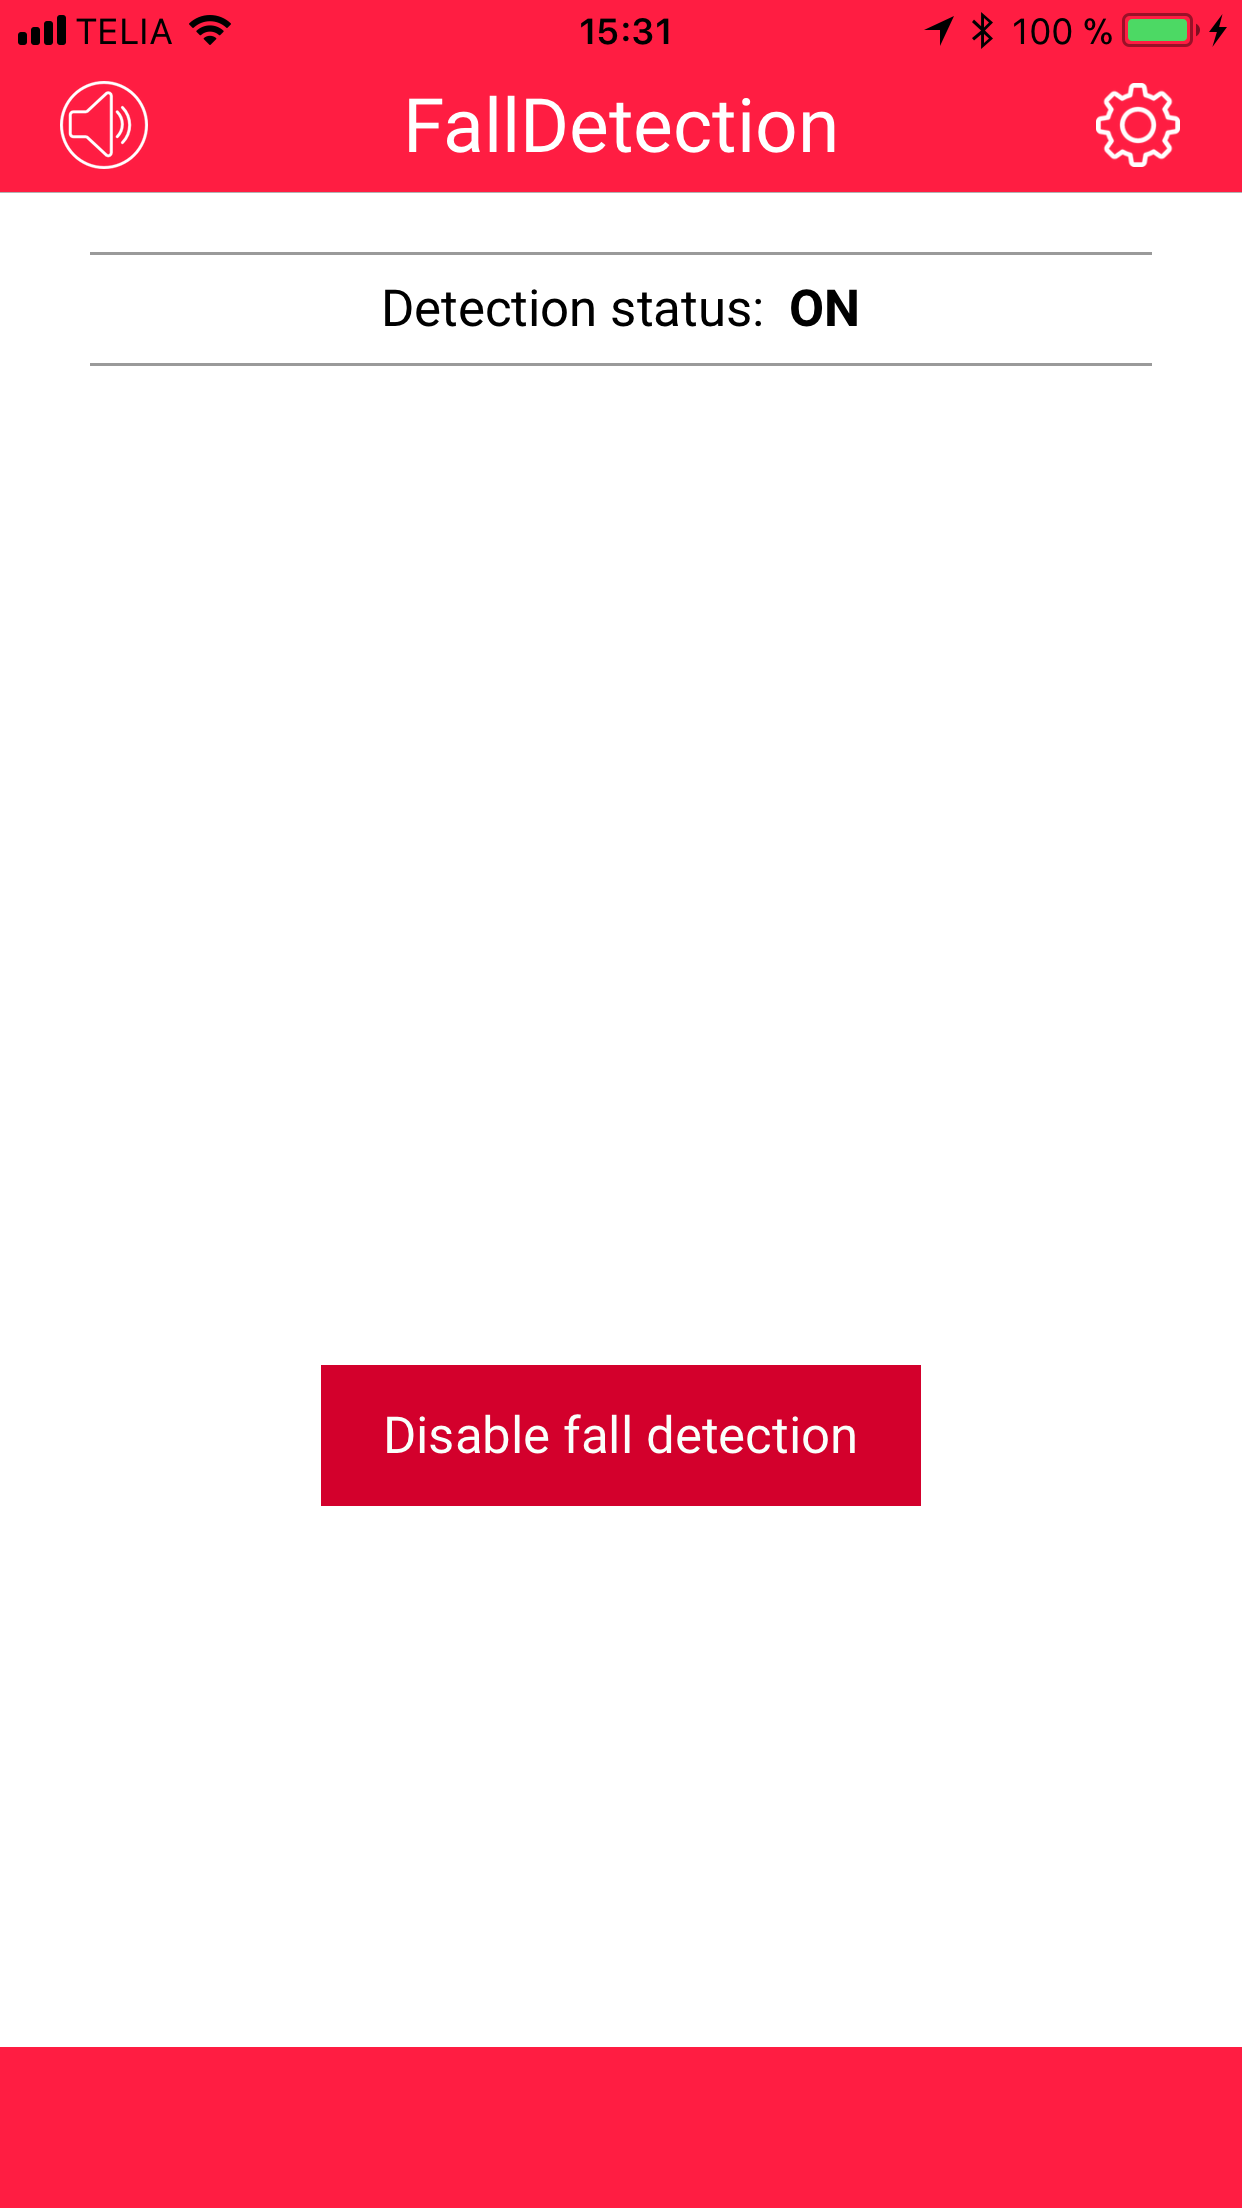
\includegraphics[width=8cm]{../img/screenshots/main-screen.jpg} }}%
		\caption{The main interface of the application lets the user enable/disable fall detection as well as got to settings and toggle sonica alarm on/off}%
		\label{fig:main-screen}%
	\end{figure}

	\begin{figure}[H]
		\centering
		\subfloat{{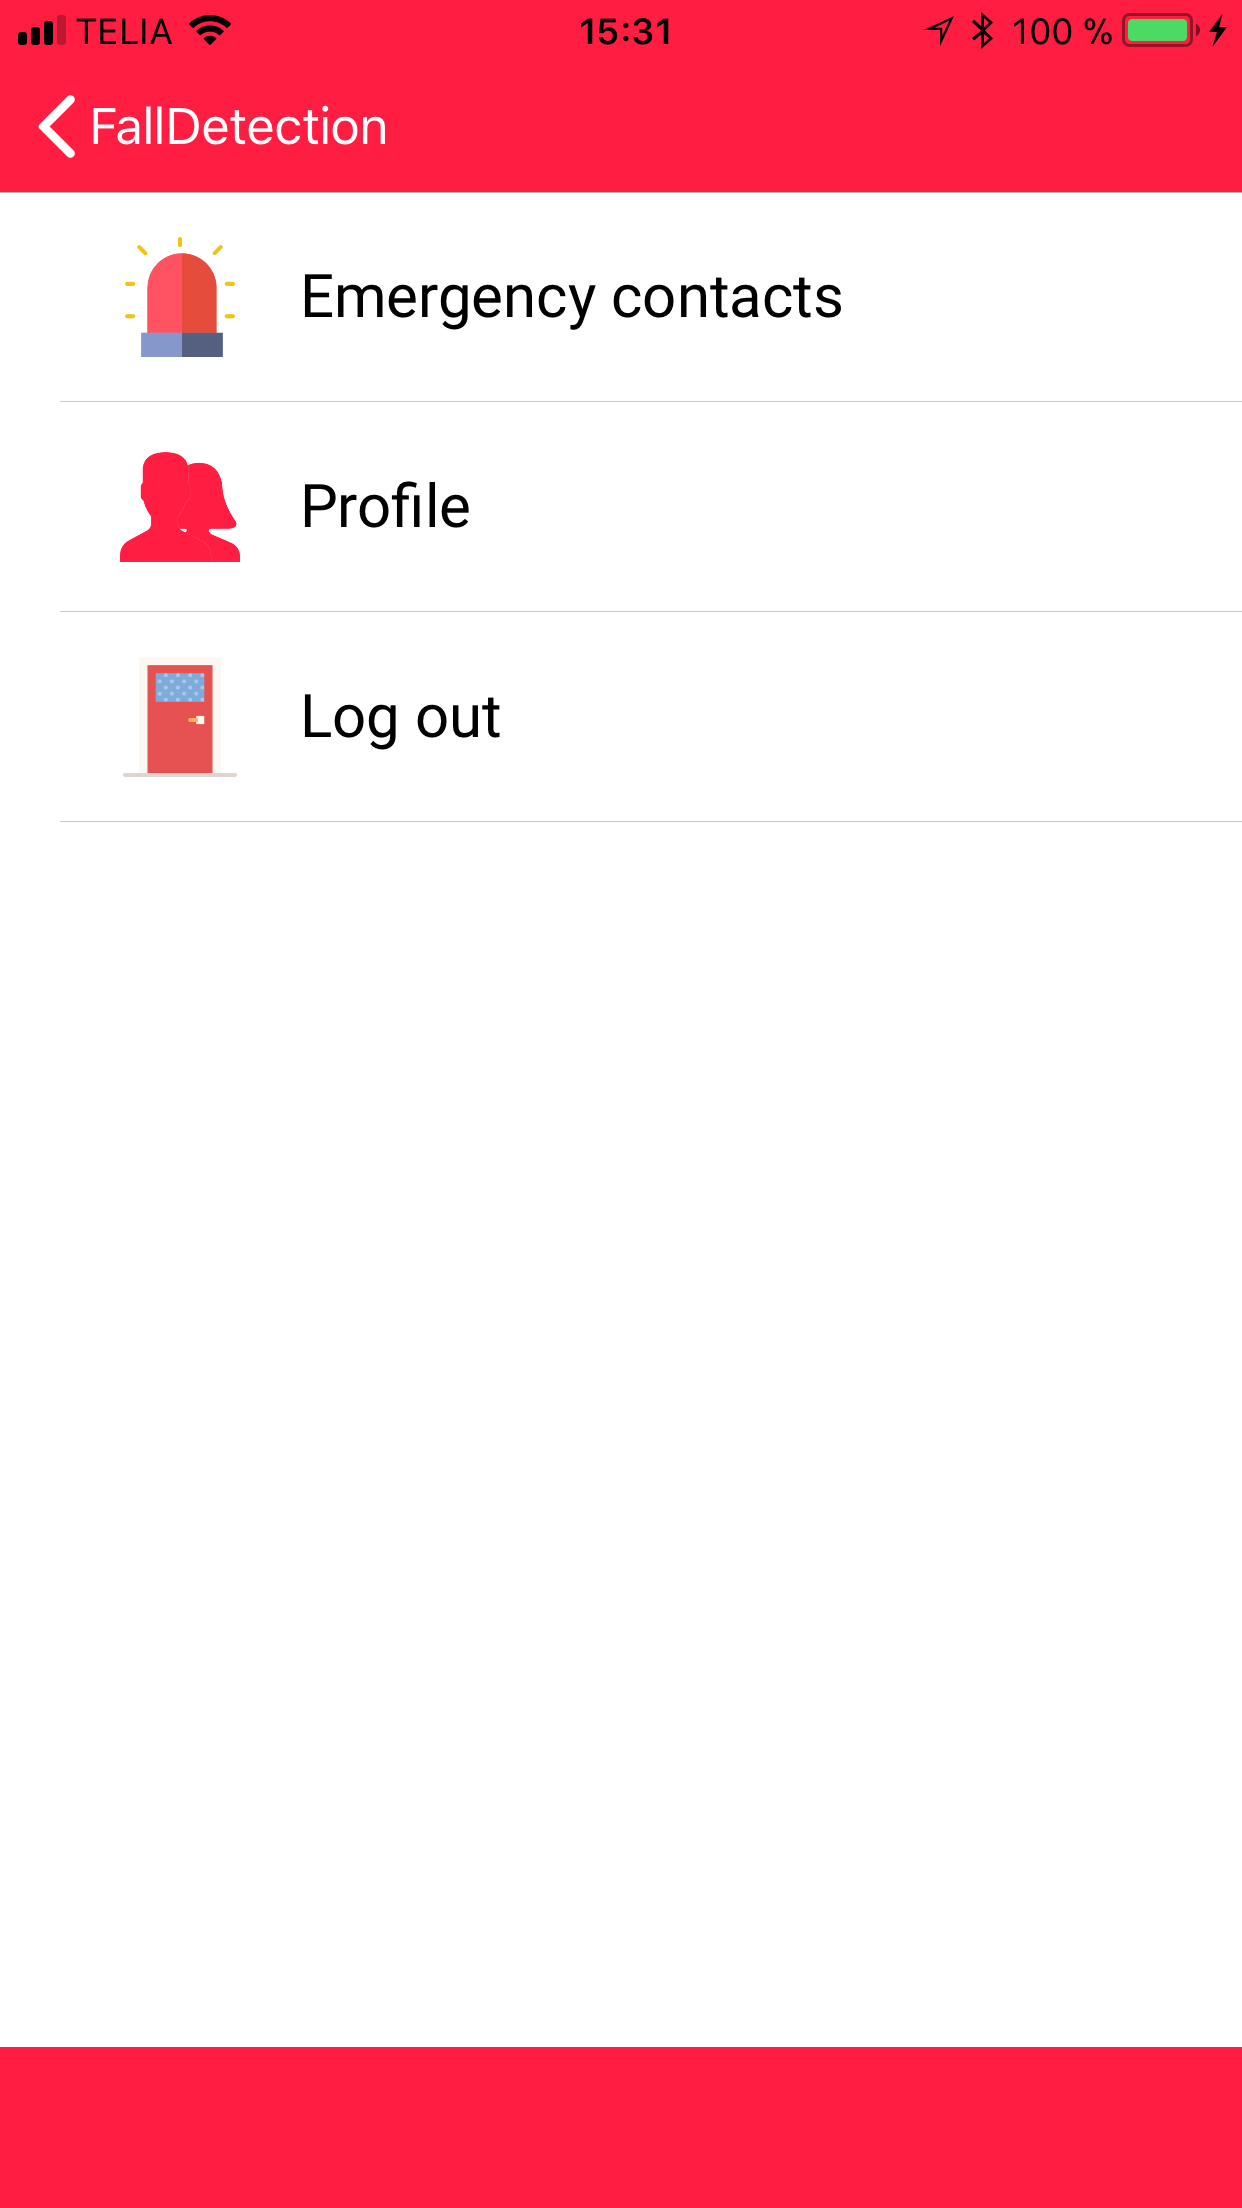
\includegraphics[width=8cm]{../img/screenshots/settings-screen.jpg} }}%
		\caption{From the settings screen, the user can choose to view emergency contacts, his or hers profile and log out of the application}%
		\label{fig:settings-screen}%
	\end{figure}
	
	\begin{figure}[H]
		\centering
		\subfloat{{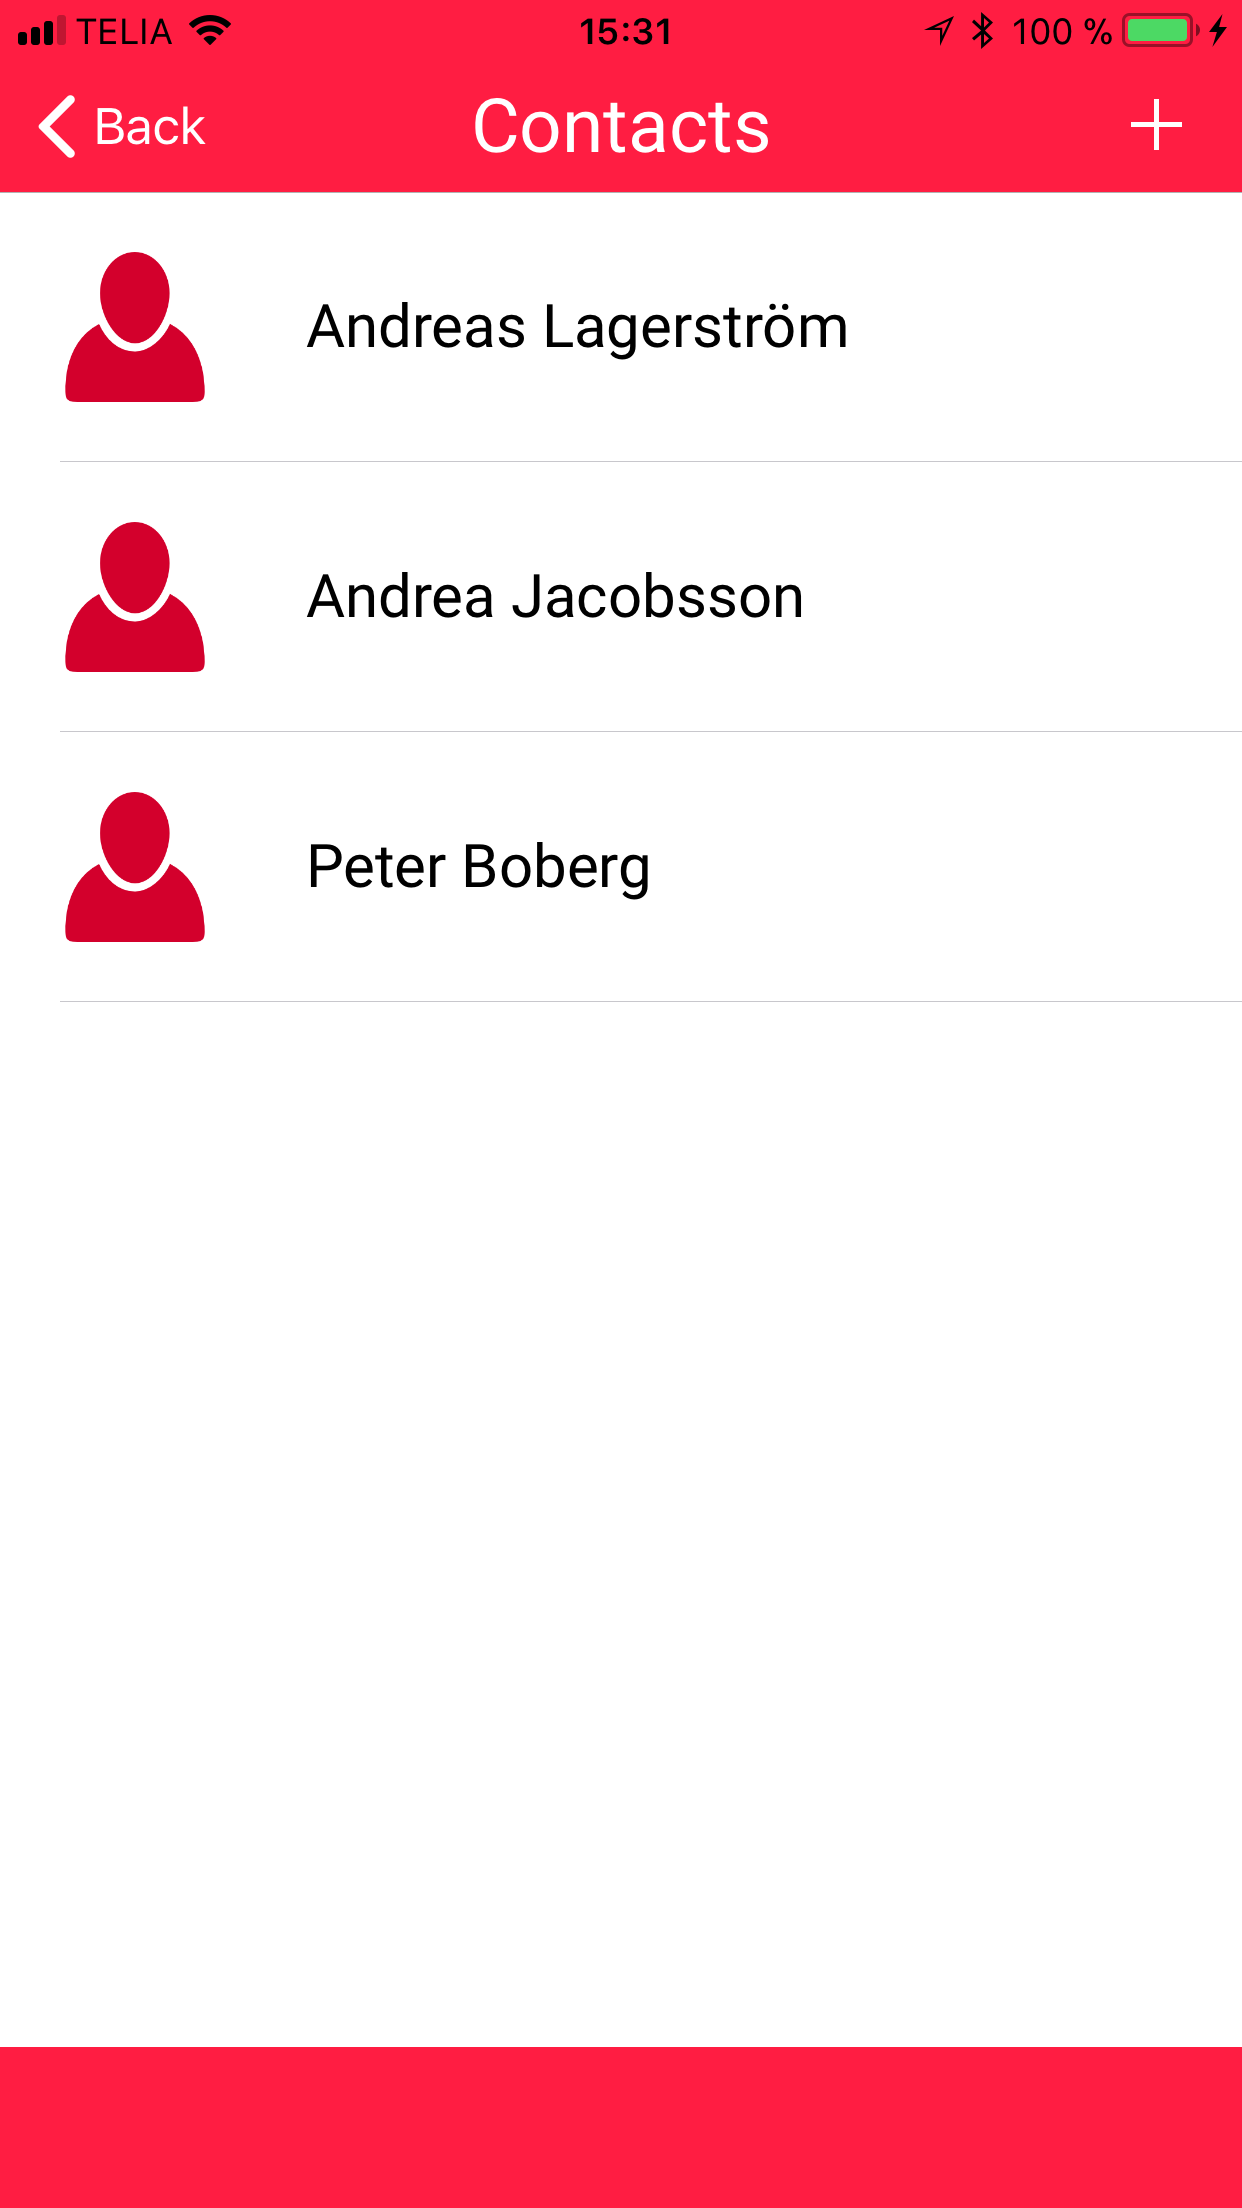
\includegraphics[width=8cm]{../img/screenshots/contacts-screen.jpg} }}%
		\caption{The contacts screen displays all emergency contacts defined by the user. The user may also add a new contact by tapping the + sign.}%
		\label{fig:contacts-screen}%
	\end{figure}

	
	\begin{figure}[H]
		\centering
		\subfloat{{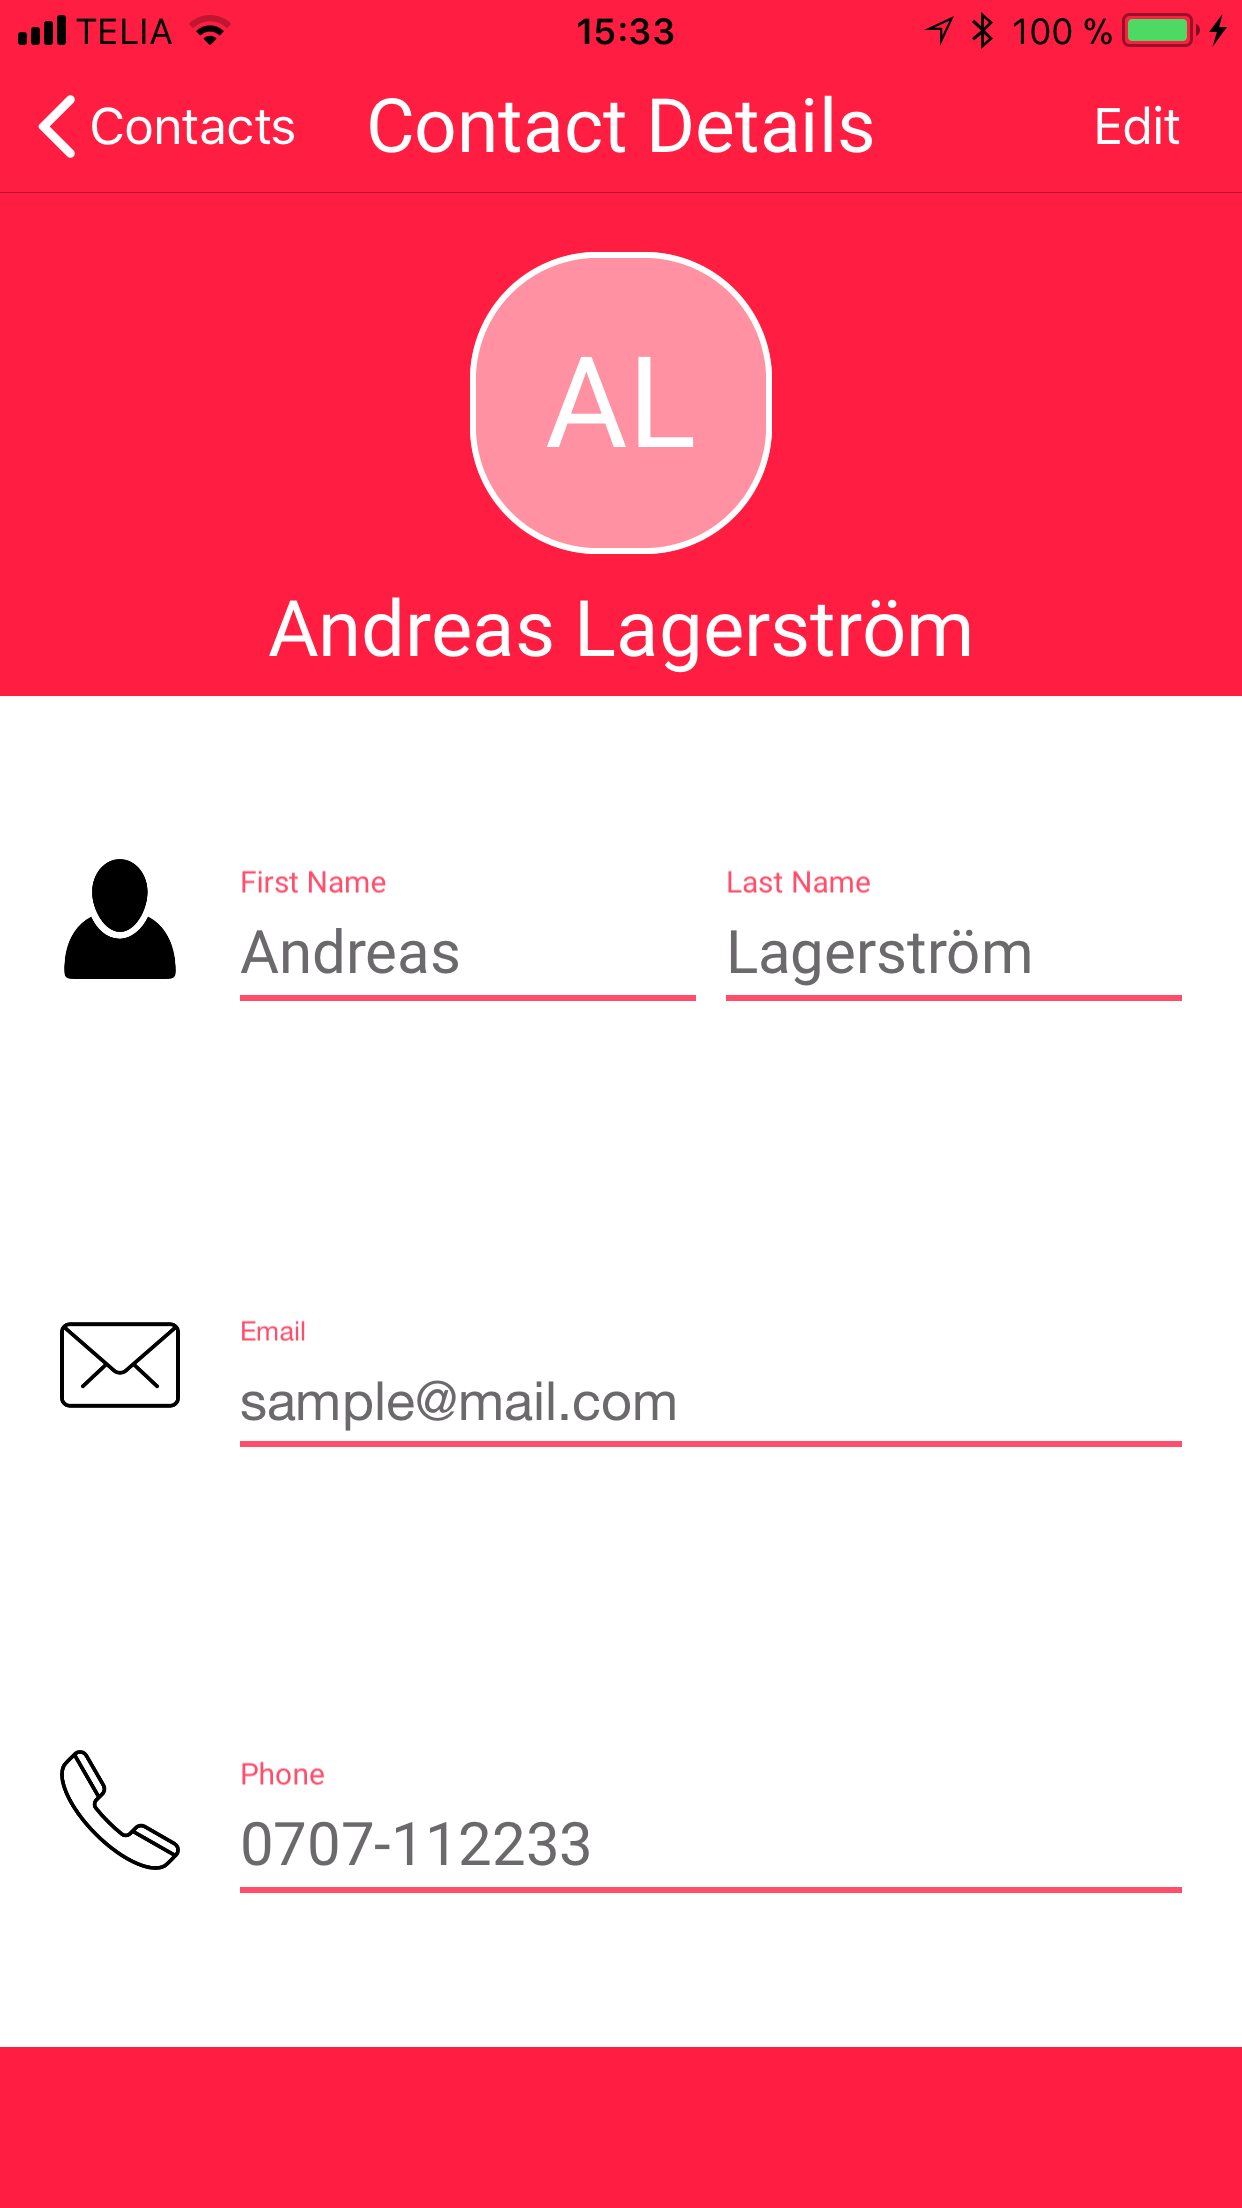
\includegraphics[width=8cm]{../img/screenshots/contacts-detail-screen.jpg} }}%
		\caption{The contact detail view let the user view contact details as well as edit them by pressing the edit button}%
		\label{fig:contacts-detail-screen}%
	\end{figure}

	\begin{figure}[H]
		\centering
		\subfloat{{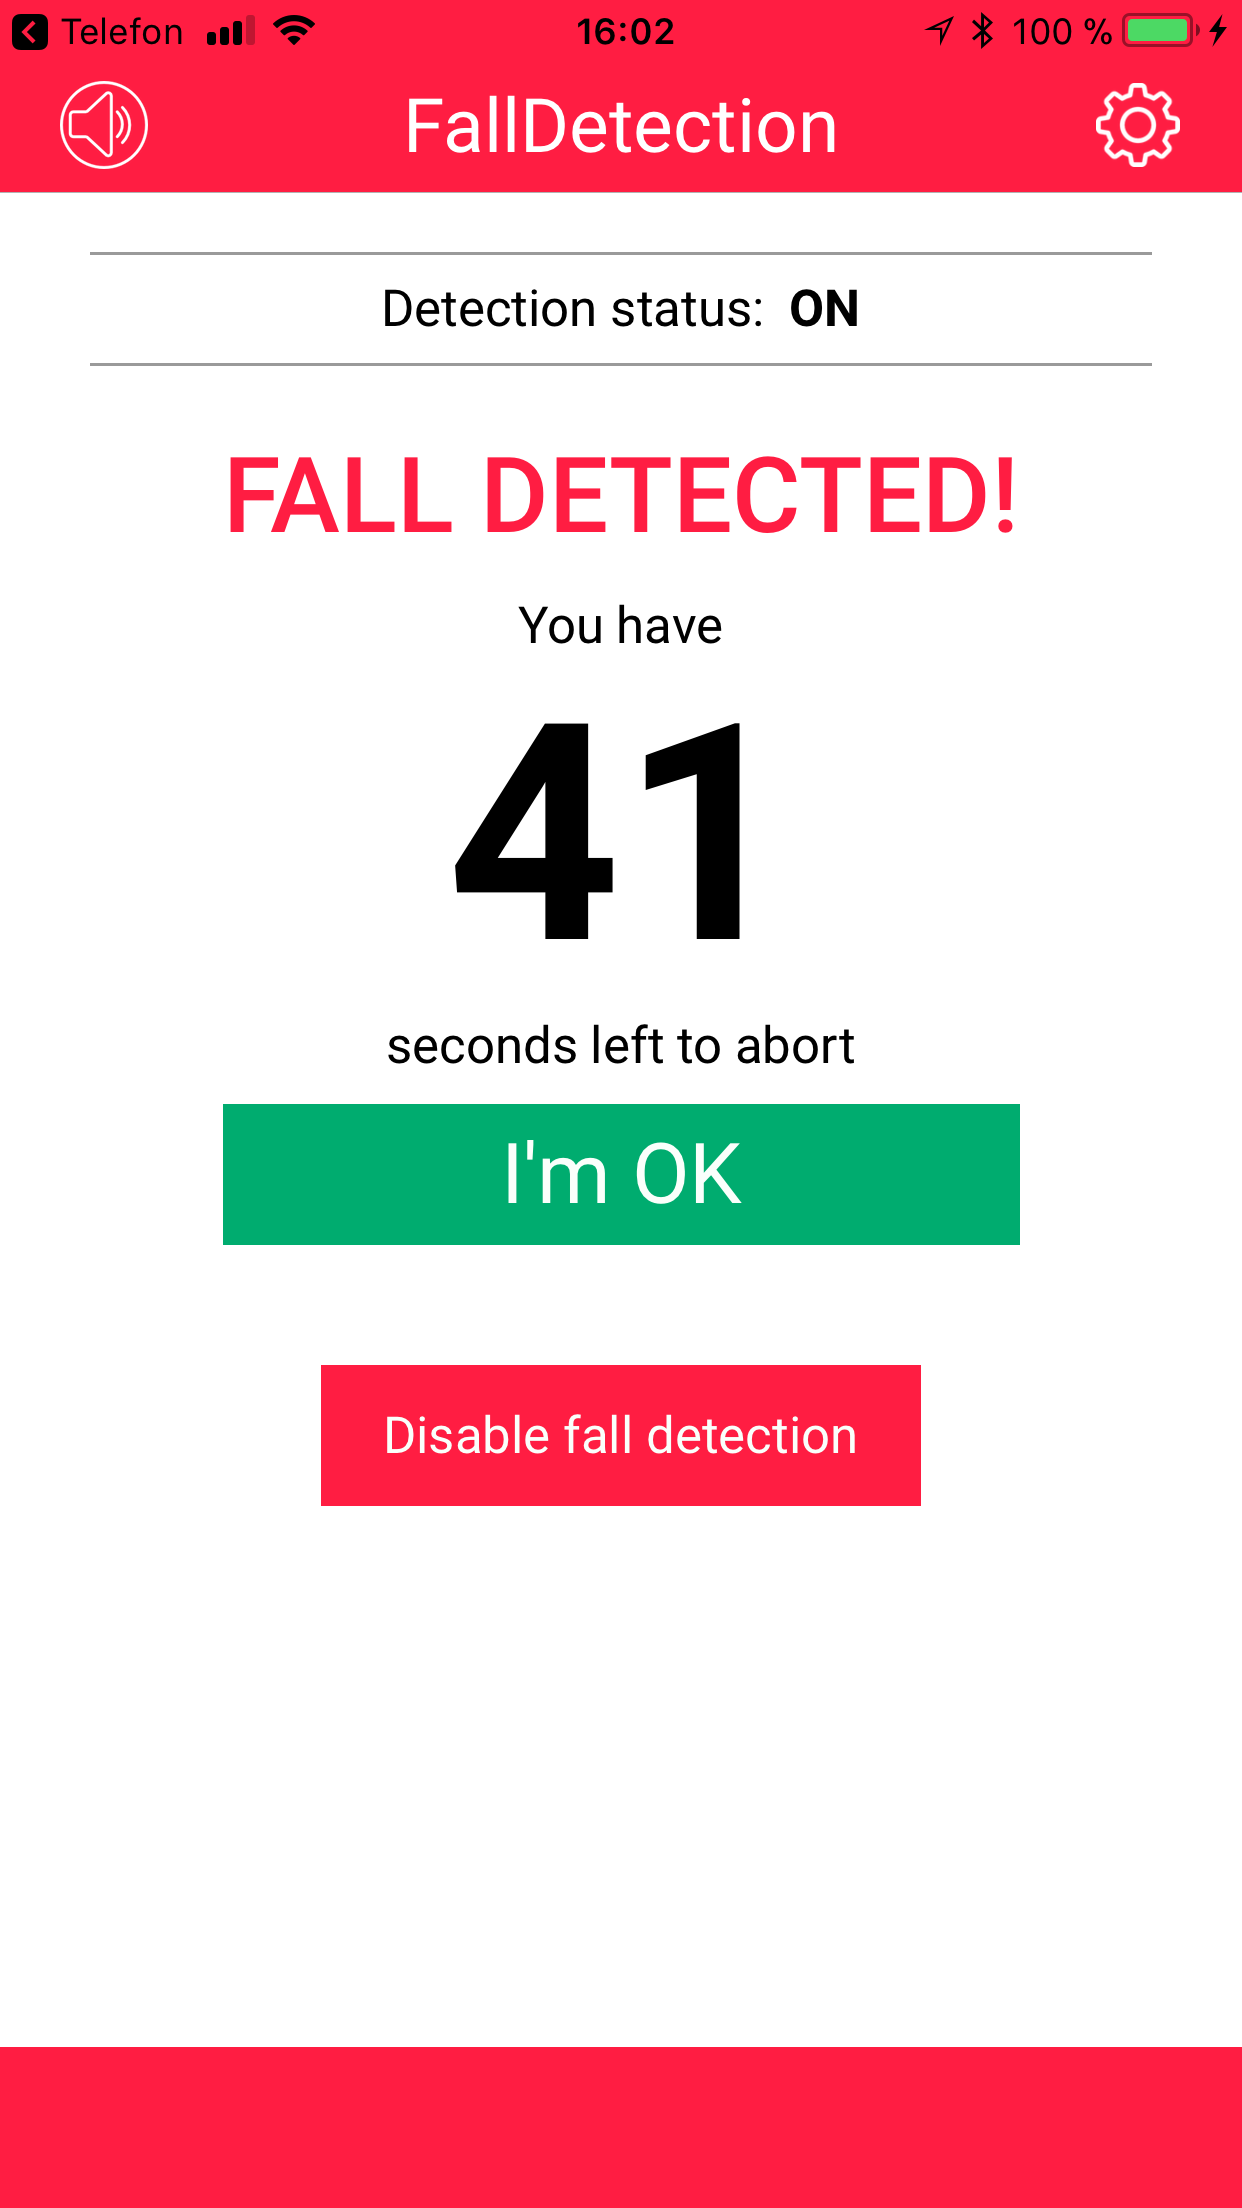
\includegraphics[width=8cm]{../img/screenshots/alarm-screen.jpg} }}%
		\caption{The alarm screen is shown when the app detects a fall, the user now has 45 seconds to discard the event by pressing "I'm OK", or an email containing information and coordinates will be sent to the users emergency contacts when the timer fires}%
		\label{fig:alarm-screen}%
	\end{figure}



		

\bibliography{bib_peter}
\bibliographystyle{ieeetr}

\end{document}